
\documentclass[12pt]{article}

\usepackage{sbc-template}
\usepackage[brazil]{babel}
\usepackage[utf8]{inputenc}
\usepackage[T1]{fontenc}
\usepackage{graphicx}
\usepackage{url}
\usepackage{booktabs}
\usepackage{array}
\usepackage{listings}
\usepackage{xcolor}

\lstset{
  basicstyle=\ttfamily\scriptsize,
  breaklines=true,
  frame=single,
  backgroundcolor=\color{gray!10},
  aboveskip=4pt,
  belowskip=4pt,
}

\sloppy

% ── Metadados ────────────────────────────────────────────────
\title{Centro de Distribuição Automatizado:\\
       Simulação Concorrente com Raylib}

\author{Artur Moraes, Helenna Massarra Paes, Pedro Calil Raposo}

\address{Instituto Brasileiro de Ensino, Desenvolvimento e Pesquisa (IDP)\\
  Ciência da Computação e Engenharia de Software\\
  Disciplina: Programação Concorrente --- 2026/1
\email{rutra2000@gmail.com, h.massarrapaes@gmail.com, pedrocalil.cordeiro@gmail.com}}

% ── Documento ────────────────────────────────────────────────
\begin{document}

\maketitle

\begin{resumo}
Este trabalho apresenta a simulação concorrente de um centro de distribuição
automatizado em C, com robôs coletores, entregadores e esteira transportadora.
A solução utiliza \textit{pthreads}, \textit{mutexes} por recurso e interface
gráfica em Raylib. O sistema foi validado em três cenários estáticos e em uma
configuração dinâmica, demonstrando entrega correta dos pacotes e ausência de
\textit{deadlocks}.
\end{resumo}

% ─────────────────────────────────────────────────────────────
\section{Organização das \textit{Threads}}
\label{sec:threads}

O programa cria $N + M + 3$ \textit{threads} POSIX \cite{posix:18} ao total,
onde $N$ é o número de robôs coletores e $M$ o de entregadores.  A Tabela~\ref{tab:threads} resume as
\textit{threads} e seus argumentos.

\begin{table}[h]
\centering
\caption{Threads do sistema}
\label{tab:threads}
\small
\begin{tabular}{llcc}
\toprule
\textbf{Thread}       & \textbf{Função}       & \textbf{Qtd.} & \textbf{Argumento}         \\
\midrule
Gerador de pacotes    & \texttt{thread\_gerador}    & 1 & \texttt{Simulacao *}       \\
Esteira               & \texttt{thread\_esteira}    & 1 & \texttt{Simulacao *}       \\
Robô coletor          & \texttt{thread\_coletor}    & N & \texttt{ArgRobo *}         \\
Robô entregador       & \texttt{thread\_entregador} & M & \texttt{ArgRobo *}         \\
Interface Raylib      & \texttt{thread\_interface}  & 1 & \texttt{Simulacao *}       \\
\bottomrule
\end{tabular}
\end{table}

Todas são criadas em \texttt{main.c} com \texttt{pthread\_create} e aguardadas
com \texttt{pthread\_join}.  A janela Raylib é aberta \emph{dentro} de
\texttt{thread\_interface} via \texttt{InitWindow}, pois a biblioteca exige
que o contexto OpenGL seja criado e usado pela mesma \textit{thread}.  O
encerramento é cooperativo: quando a flag \texttt{sim.rodando} vai a zero,
todos os laços terminam naturalmente e os \texttt{pthread\_join} retornam.

% ─────────────────────────────────────────────────────────────
\section{Recursos Compartilhados}
\label{sec:recursos}

A Tabela~\ref{tab:recursos} lista os recursos compartilhados e seus acessores.

\begin{table}[ht]
\centering
\caption{Recursos compartilhados do sistema}
\label{tab:recursos}
\footnotesize
\begin{tabular}{>{\raggedright\arraybackslash}p{4.1cm}
                >{\raggedright\arraybackslash}p{2.4cm}
                >{\raggedright\arraybackslash}p{6.6cm}}
\toprule
\textbf{Recurso} & \textbf{Tipo} & \textbf{Acessado por} \\
\midrule
\texttt{Mapa.celulas[]}\allowbreak\texttt{.ocupante} &
  grade de células &
  todos os robôs (r/w de posição) e interface (leitura) \\
\addlinespace
\texttt{Esteira.posicoes[]} &
  buffer linear &
  coletores (inserção), esteira (avanço), entregadores (retirada), interface \\
\addlinespace
\texttt{Estacao} (\texttt{cabeca}, \texttt{cauda}, \texttt{quantidade}) &
  fila encadeada &
  gerador (enfileira) e coletores (desenfileira) \\
\addlinespace
\texttt{Estatisticas} &
  contadores inteiros &
  gerador e entregadores (escrita); interface (leitura) \\
\addlinespace
\texttt{Simulacao.rodando} &
  flag de parada &
  qualquer \textit{thread} pode escrever; todas leem \\
\bottomrule
\end{tabular}
\end{table}

% ─────────────────────────────────────────────────────────────
\section{Seções Críticas Identificadas}
\label{sec:criticas}

\textbf{Movimentação de robôs (\texttt{mapa.c}).}
Dois robôs podem tentar ocupar a mesma célula simultaneamente.
\texttt{mapa\_tenta\_mover} adquire \texttt{Mapa.mutex}, verifica se o destino
está livre, atualiza origem e destino e libera o \textit{mutex} em um único
\textit{lock}, garantindo exclusão mútua.

\textbf{Esteira (\texttt{esteira.c}).}
O vetor \texttt{posicoes[]} é acessado por três \textit{threads}: inserção em
\texttt{[0]}, avanço de \texttt{[i-1]} para \texttt{[i]} e retirada em
\texttt{[tamanho-1]}.  Todas as operações adquirem \texttt{Esteira.mutex}
antes de qualquer acesso.

\textbf{Filas de estações (\texttt{estacao.c}).}
Gerador e múltiplos coletores disputam a mesma estação: enfileirar e
desenfileirar adquirem \texttt{Estacao.mutex}, garantindo que lista encadeada
e contador sejam modificados atomicamente.

\textbf{Estatísticas (\texttt{simulacao.c}).}
\texttt{stats\_inc\_entregues} incrementa e testa a meta \emph{sob o mesmo
lock}; atingida, libera o \textit{lock} e chama \texttt{simulacao\_parar}. O
teste atômico evita parada duplicada por corrida.

% ─────────────────────────────────────────────────────────────
\section{Mecanismos de Sincronização}
\label{sec:sync}

\textbf{\texttt{pthread\_mutex\_t} --- exclusão mútua por recurso.}
Cada recurso possui seu próprio \textit{mutex} (\texttt{Mapa.mutex},
\texttt{Esteira.mutex}, \texttt{Estacao.mutex} por estação,
\texttt{Estatisticas.mutex}).  A granularidade fina permite que \textit{threads}
que acessam recursos distintos avancem em paralelo.  Nenhuma \textit{thread}
adquire dois \textit{locks} simultaneamente, eliminando o risco de \textit{deadlock}
por espera circular.

\textbf{\texttt{volatile sig\_atomic\_t rodando} --- flag de término.}
\texttt{volatile} impede que o compilador cache o valor em registrador.
Formalmente, \texttt{sig\_atomic\_t} garante atomicidade apenas frente a
\textit{signal handlers}, não entre \textit{threads}; a corretude aqui
apoia-se em cargas e armazenamentos alinhados serem atômicos em x86-64 e na
flag transitar uma única vez, de \texttt{1} para \texttt{0}.  O pior caso é
uma \textit{thread} executar um \textit{tick} extra após a parada ---
aceitável nesta simulação.  Uma alternativa estritamente portável seria
\texttt{\_Atomic int} de \texttt{stdatomic.h} (C11).

\textbf{Espera ativa com \texttt{dormir\_ms}.}
Nos pontos de espera (coletor aguardando espaço na esteira; entregador
aguardando pacote na saída), as \textit{threads} dormem \texttt{passo\_ms} e
tentam novamente.  Como o intervalo entre tentativas é limitado por
\texttt{passo\_ms} --- o período que dita o ritmo da simulação ---, o custo do
\textit{polling} é desprezível: no máximo uma verificação por \textit{tick},
sem consumo de CPU entre elas.  \texttt{pthread\_cond\_t} reduziria a latência
de notificação, mas ela já é mascarada pelo próprio passo da simulação.

% ─────────────────────────────────────────────────────────────
\section{Decisões de Projeto}
\label{sec:projeto}

\textbf{Interface gráfica com Raylib (bônus +10\%).}
O enunciado prevê \textit{ncurses} como padrão e oferece bônus para grupos que
substituam integralmente a interface por Raylib \cite{raylib}.  Este projeto
implementa a interface com Raylib: o mapa é renderizado como grade de células
coloridas e o painel lateral exibe esteira, contadores e progresso em tempo
real (Figura~\ref{fig:interface}).  A \textit{thread} de interface captura um
\textit{snapshot} do estado sob \textit{mutex} e renderiza em seguida, sem
manter recursos travados durante o desenho.

\begin{figure}[ht]
\centering
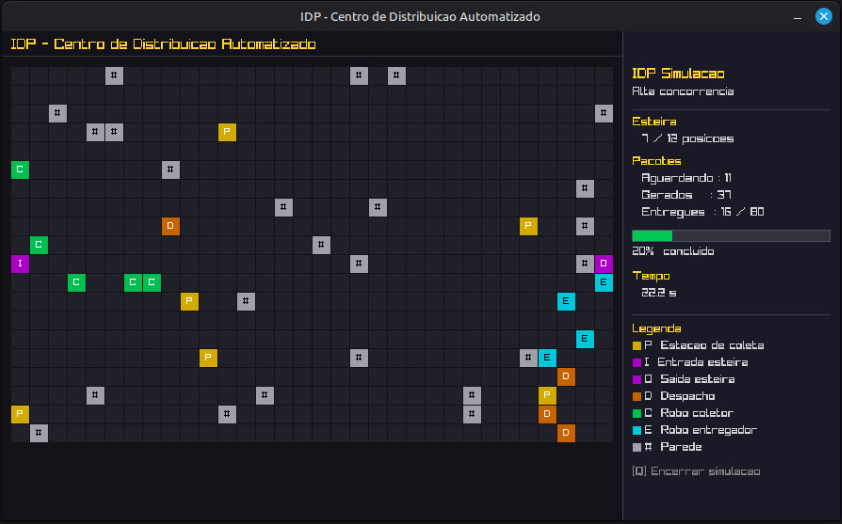
\includegraphics[height=2.6cm]{interface-alta.png}\hspace{4mm}%
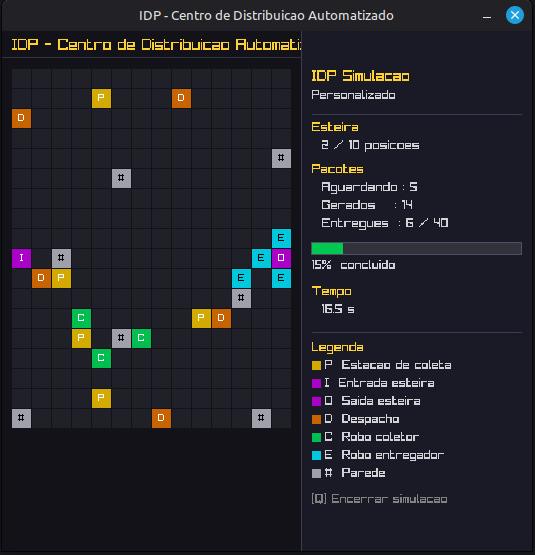
\includegraphics[height=2.6cm]{interface-dinamico.png}
\caption{Interface Raylib nos cenários Alta Concorrência (esq.) e
  Personalizado/dinâmico (dir.).}
\label{fig:interface}
\end{figure}

\textbf{Mutex por recurso em vez de mutex global.}
Um \textit{mutex} global criaria gargalo: a interface bloquearia todos os
robôs durante a renderização.  Com \textit{mutexes} por recurso, cada robô
bloqueia apenas a célula que tenta ocupar, e a interface segura
\texttt{Mapa.mutex} apenas durante uma cópia de buffer.

\textbf{BFS com leitura \textit{lock-free}.}
Cada passo recalcula o BFS \cite{cormen:09} lendo \texttt{ocupante} sem
\textit{mutex}.  Dados desatualizados apenas fazem o robô tentar um passo que
falha em \texttt{mapa\_tenta\_mover} (atômico); o próximo ciclo recalcula.
Isso elimina contenção no \textit{mutex} do mapa durante o planejamento.

\textbf{Heurística gulosa para escolha de destino.}
Coletores escolhem a estação \emph{não-vazia mais próxima} (distância de
Manhattan); entregadores, o \emph{despacho mais próximo}.  Não é ótimo
globalmente, mas distribui robôs entre estações/despachos sem comunicação
entre \textit{threads}.

\textbf{Lógica \texttt{afastar\_da\_entrada}.}
Coletores ociosos junto à entrada da esteira poderiam bloquear o último
coletor carregado.  A função move o coletor ocioso para a célula vizinha mais
distante da entrada, liberando o gargalo.

% ─────────────────────────────────────────────────────────────
\section{Guia de Utilização}
\label{sec:uso}

A interface exige Raylib 5.5. No Ubuntu 24.04, a biblioteca pode ser
instalada a partir do fonte:

\begin{lstlisting}[language=bash]
sudo apt install build-essential git libasound2-dev libx11-dev \
  libxrandr-dev libxi-dev libgl1-mesa-dev libglu1-mesa-dev \
  libxcursor-dev libxinerama-dev libwayland-dev libxkbcommon-dev
git clone --depth 1 --branch 5.5 https://github.com/raysan5/raylib.git
cd raylib/src && make PLATFORM=PLATFORM_DESKTOP && sudo make install
\end{lstlisting}

Alternativamente, o \texttt{Dockerfile} incluso constrói imagem pronta
(\texttt{podman build -t idp\_sim .}), executável montando
\texttt{/tmp/.X11-unix} e exportando \texttt{DISPLAY}.  Com a biblioteca
disponível:

\begin{lstlisting}[language=bash]
make                # compila ./idp_sim
./idp_sim 1         # Cenario Simples       (18x12, 20 pacotes)
./idp_sim 2         # Cenario Intermediario (24x16, 40 pacotes)
./idp_sim 3         # Alta Concorrencia     (32x20, 80 pacotes)
./idp_sim 0         # Configuracao dinamica (le parametros)
make teste teste-bfs teste-stress   # testes automatizados
# tecla Q encerra a simulacao antecipadamente
\end{lstlisting}

% ─────────────────────────────────────────────────────────────
\section{Resultados}
\label{sec:resultados}

Os três cenários estáticos e a configuração dinâmica foram executados em
Ubuntu 24.04; a Tabela~\ref{tab:resultados} resume os resultados.  O cenário
dinâmico usou parâmetros não-padrão (5 estações, 5 despachos, 7 obstáculos,
esteira de 10, \textit{tick} de 250\,ms), exercitando o leitor de configuração.

\begin{table}[ht]
\centering
\caption{Resultados observados por cenário}
\label{tab:resultados}
\small
\begin{tabular}{lcccccc}
\toprule
\textbf{Cenário} & \textbf{Mapa} & \textbf{Pacotes} & \textbf{Colet.} &
\textbf{Entreg.} & \textbf{Entregues} & \textbf{Tempo (s)} \\
\midrule
1 --- Simples           & $18\times12$ & 20 & 2 & 1 & 20/20 & 76,2 \\
2 --- Intermediário     & $24\times16$ & 40 & 3 & 2 & 40/40 & 83,8 \\
3 --- Alta Concorrência & $32\times20$ & 80 & 4 & 4 & 80/80 & 92,5 \\
0 --- Dinâmico          & $14\times18$ & 40 & 3 & 4 & 40/40 & 65,0 \\
\bottomrule
\end{tabular}
\end{table}

Em todas as execuções, a totalidade dos pacotes foi entregue e a simulação
encerrou de forma limpa, com todos os \texttt{pthread\_join} retornando.
Não foram observados \textit{deadlocks} nem corrupção de estado: nenhum robô
ocupou célula já ocupada, nenhum pacote foi perdido ou duplicado na esteira,
e as estatísticas fecharam consistentes com o total gerado.

No Cenário 3 observou-se maior disputa pelas células adjacentes à entrada da
esteira; a lógica \texttt{afastar\_da\_entrada} (Seção~\ref{sec:projeto})
mostrou-se necessária para evitar bloqueio do último coletor carregado.  Os
testes automatizados passaram em todas as execuções, incluindo repetições
consecutivas para exercitar intercalações distintas de \textit{threads}.

% ─────────────────────────────────────────────────────────────
\section{Conclusão}
\label{sec:conclusao}

Este trabalho implementou um centro de distribuição automatizado como sistema
concorrente em C, com entidades modeladas por \textit{threads} POSIX. A adoção
de um \textit{mutex} por recurso, seções críticas curtas e ausência de
\textit{locks} aninhados garantiu exclusão mútua sem \textit{deadlocks}.

Os testes confirmaram a entrega correta dos pacotes, o encerramento cooperativo
e a estabilidade do sistema mesmo sob alta concorrência. Como melhorias futuras,
destacam-se o uso de \texttt{stdatomic.h}, variáveis de condição e políticas de
roteamento cooperativas para reduzir contenção.
% ─────────────────────────────────────────────────────────────
\begin{thebibliography}{9}

\bibitem{raylib}
Santamaria, R. (2013--2025).  \textit{raylib}.
\url{https://www.raylib.com}.

\bibitem{posix:18}
IEEE and The Open Group (2018).  \textit{IEEE Std 1003.1-2017 --- Portable
Operating System Interface (POSIX)}.  IEEE, New York.

\bibitem{cormen:09}
Cormen, T. H., Leiserson, C. E., Rivest, R. L., and Stein, C. (2009).
\textit{Introduction to Algorithms}, 3rd ed.  MIT Press.

\end{thebibliography}

\end{document}